% vim: expandtab tabstop=2 softtabstop=2 shiftwidth=2
\documentclass[aspectratio=169]{beamer}
\usepackage[portuguese]{babel}

\usepackage{beamerx}
\usepackage{hyperref}
\hypersetup{colorlinks,linkcolor={blue},citecolor={blue},urlcolor={blue}}

\usepackage{lmodern}			% Usa a fonte Latin Modern
\usepackage[T1]{fontenc}		% Selecao de codigos de fonte.
\usepackage[utf8]{inputenc}		% Codificacao do documento (conversão automática dos acentos)
\usepackage{indentfirst}		% Indenta o primeiro parágrafo de cada seção.
\usepackage{color}				% Controle das cores
\usepackage{graphicx}			% Inclusão de gráficos
\usepackage{microtype} 			% para melhorias de justificação
\usepackage{epigraph}
\usepackage{tcolorbox}
\usepackage{hyperref}
\usepackage{pgfgantt}
\usepackage{booktabs}
\usepackage{multirow}
\usepackage{tikz}
\usepackage{enumitem}
\usepackage{amsmath}
\usepackage{amssymb}
\usepackage{amsfonts}
\usepackage{mathtools}
\usepackage{caption}
\usepackage{subcaption}
\usepackage{circuitikz}
\usepackage{algorithm2e}
\RestyleAlgo{ruled}
\usetikzlibrary{chains, positioning, shadows, arrows.meta, calc, shapes.geometric}
\tikzset{
    block/.style={
        rectangle,
        rounded corners,
        draw=black, thick,
        text width=4.5em,
        minimum height=3em,
        align=center
    },
    arrow/.style={->, thick}
}
\usepackage[table]{xcolor}

\title[PSI5844: Projeto e implementação de radares microondas]
      {Filtro passa-baixas em microstrip}
      []

\author{
\textbf{Gabriel Pereira de Carvalho} \\
\textbf{Heitor Albuquerque}
}

% Dissertação discute 2 topologias de LPF em microlinha
% 1) Filtro passa-baixas de impedância em escada (vamos focar nessa!)
% 2) Filtro de linhas acopladas paralelas

%\xsectionframe{themeturquoise-bg}{themeturquoise-altbg}{themeturquoise-fg}{salab2.jpg}{}{}
%\xsectionframe{themeturquoise-bg}{themeturquoise-altbg}{themeturquoise-fg}{poliFormatura.jpg}{}{}

\setcolortheme{blue}

\begin{document}
\maketitle

\xsectionframe{themeturquoise-bg}{themeturquoise-altbg}{themeturquoise-fg}{pei.jpg}{Filtro passa-baixas de impedância em escada}{}

\begin{frame}{}
\begin{figure}
    \centering
    \caption{Topologia do filtro "high Z, low Z"}
    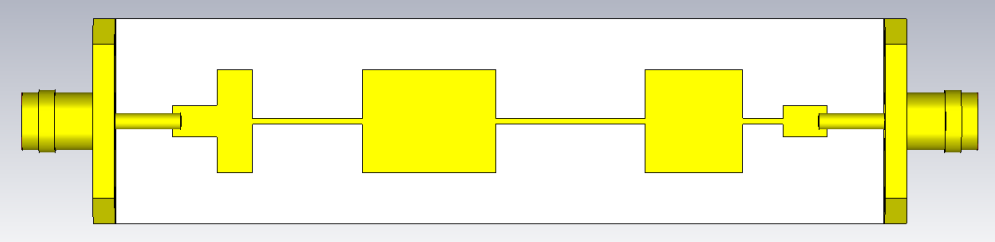
\includegraphics[width=.8\textwidth]{images/escada.png}
    \label{fig:escada}
    \par\vspace{0.01cm}
    {\footnotesize \raggedright Fonte: \cite{vasco2020}\par}
\end{figure}
\begin{itemize}
    \item $Z_l = 20\Omega < 50\Omega = Z_0 \implies$ microstrip mais espessa com comportamento capacitivo
    \item $Z_h = 120\Omega > 50\Omega = Z_0 \implies$ microstrip mais fina com comportamento indutivo
\end{itemize}
\end{frame}

\begin{frame}{}
\begin{figure}
    \centering
    \caption{Etapas de design do LPF com microstrip}
    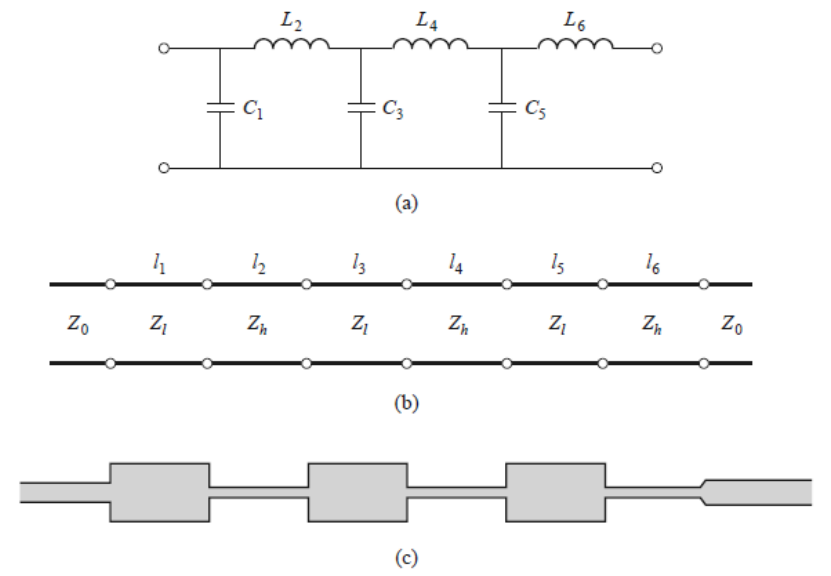
\includegraphics[height=.8\paperheight]{images/lumped_to_microstrip.png}
    \label{fig:escada}
    \par\vspace{0.01cm}
    {\footnotesize \raggedright Fonte: \cite{vasco2020}\par}
\end{figure}
\end{frame}

% It is difficult to realize filters beyond 500 MHz using lumped elements because the physical
% dimensions of the filter become comparable to the wavelength which in turns causes different
% losses that degrade the performance of the circuit. Consequently, the lumped element filters
% should be converted into distributed element realizations. To convert lumped elements
% into distributed elements, Richard’s transforms is used. At microwave frequencies, the distance
% between components is not negligible and to solve for such a problem, Kuroda’s identities are
% used for separating filter elements by inserting transmission line sections.

\begin{frame}{}
\begin{figure}
    \centering
    \caption{Transformação de Richard}
    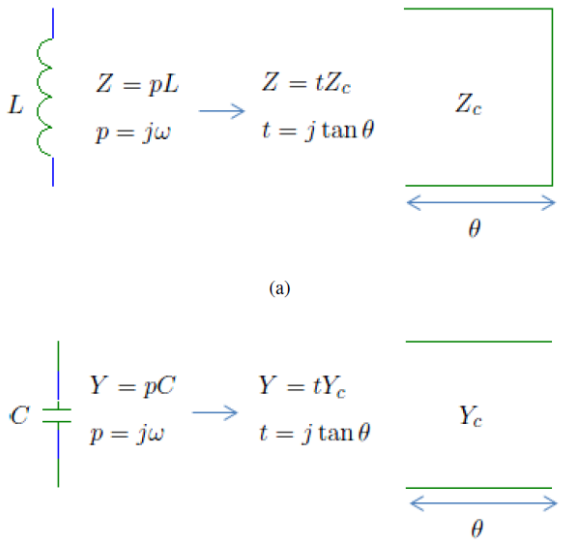
\includegraphics[height=.8\paperheight]{images/richard.png}
    \label{fig:escada}
    \par\vspace{0.01cm}
    {\footnotesize \raggedright Fonte: \cite{vasco2020}\par}
\end{figure}
\end{frame}

\begin{frame}{}
\begin{figure}
    \centering
    \caption{Transformação de Kuroda}
    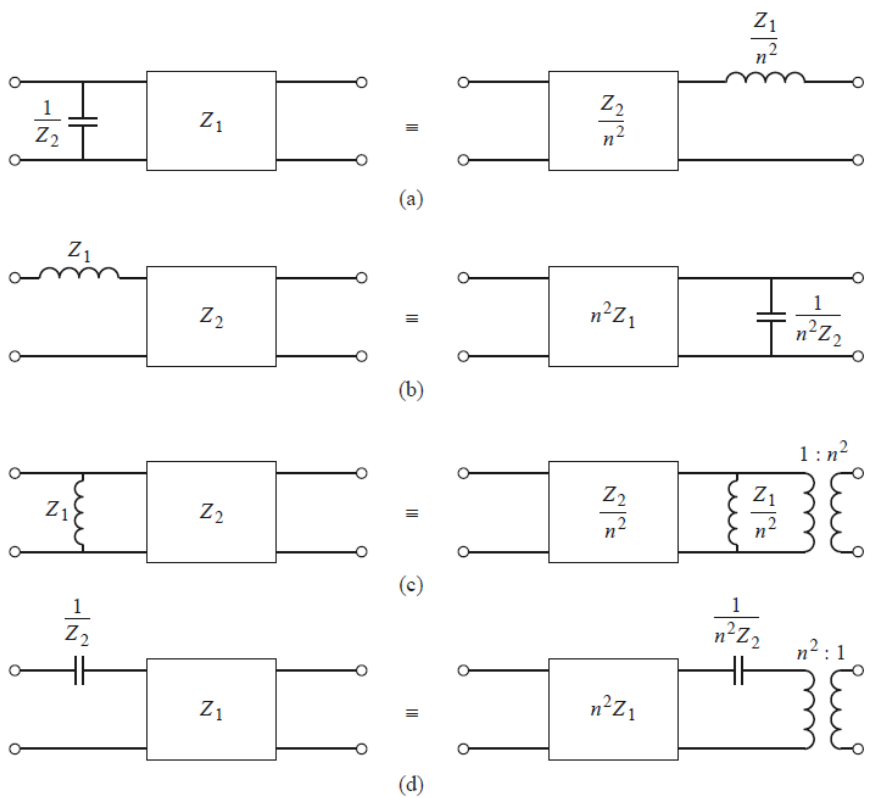
\includegraphics[height=.8\paperheight]{images/kuroda.png}
    \label{fig:escada}
    \par\vspace{0.01cm}
    {\footnotesize \raggedright Fonte: \cite{vasco2020}\par}
\end{figure}
\end{frame}

\xsectionframe{themeturquoise-bg}{themeturquoise-altbg}{themeturquoise-fg}{welcome.jpg}{Schematic e simulação no ADS}{}

\begin{frame}{Filtro base}
\textbf{\large Butterworth passa-baixas de ordem 3}
\begin{align*}
    \begin{cases}
        C_i &= \frac{1}{\pi f_c R} \sin\left(\frac{(2i - 1)\pi}{2n}\right) \quad \text{para } i=1,3,5,\ldots\\
        L_i &= \frac{R}{\pi f_c} \sin\left(\frac{(2i - 1) \pi}{2n}\right) \quad \text{para } i=2,4,6,\ldots
    \end{cases}
\end{align*}
\textbf{\large Electrical length $E_{\mathrm{eff}}$}
\begin{align*}
    \begin{cases}
        \beta l_L &= \frac{L \omega_c}{Z_h}\\
        \beta l_C &= C \omega_c Z_l
    \end{cases}
\end{align*}
\begin{table}[h]
    \begin{tabular}{|c|c|c|c|c|}
        \hline
        & & $\beta l$ & Comprimento & Espessura $w_h$,$w_l$ \\
        \hline
        $C_1$ & $9,1$pF & $57,3^\circ$ & $13,22$mm & $8,15$mm \\
        \hline
        $L_2$ & $45$nH & $114,6^\circ$  & $31,25$mm & $0,44$mm \\
        \hline
        $C_3$ & $9,1$pF & $57,3^\circ$ & $13,22$mm & $8,15$mm \\
        \hline
    \end{tabular}
\end{table}
\href{https://www.arkrfsystems.com/Linecalc.htm}{https://www.arkrfsystems.com/Linecalc.htm}
\end{frame}

\begin{frame}
\begin{figure}
    \centering
    \caption{Schematic no ADS}
    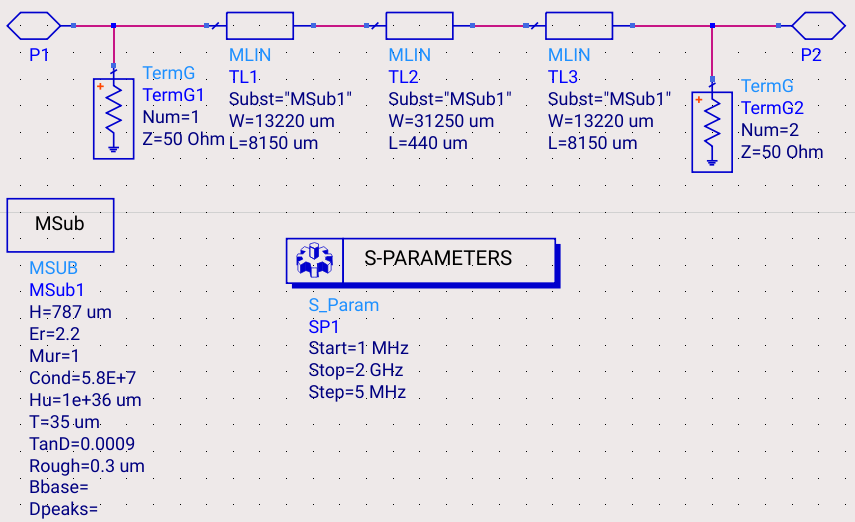
\includegraphics[height=.7\paperheight]{images/ads_schematic.png}
    \label{fig:escada}
    \par\vspace{0.01cm}
    {\footnotesize \raggedright Fonte: os autores\par}
\end{figure}
\end{frame}

\begin{frame}
Inicialmente temos $\omega_c \approx 1,2$GHz.

Utilizar \textit{parameter tuning} para obter $\omega_c \approx 350$MHz ?

\begin{figure}
    \centering
    \caption{Forward Transmission Coefficient $S(2,1)$}
    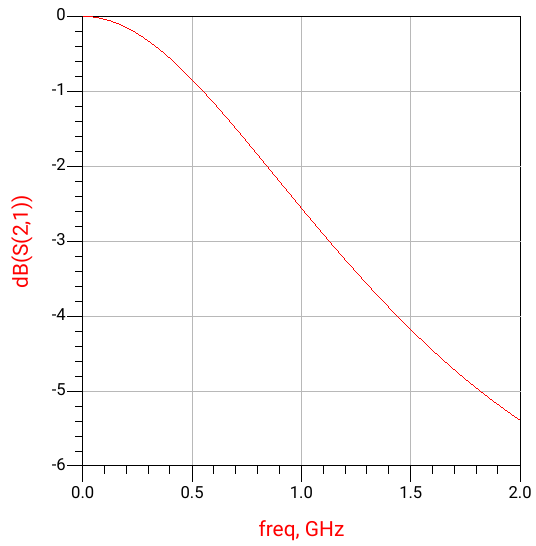
\includegraphics[height=.55\paperheight]{images/filtro.png}
    \label{fig:escada}
    \par\vspace{0.01cm}
    {\footnotesize \raggedright Fonte: os autores\par}
\end{figure}
\end{frame}

\begin{frame}[allowframebreaks]
  \frametitle{Referências Bibliográficas}
  \bibliographystyle{amsalpha}
  \bibliography{refs.bib}
\end{frame}

\end{document}
